\documentclass[11pt,a4paper]{article}
\usepackage[utf8]{inputenc}
\usepackage{graphicx}
\usepackage[margin=1in]{geometry}

\title{Wireshark}
\author{
David Zwart (4224582, dzwart@student.tudelft.nl) \\
Joseph Verburg (4018575, j.p.verburg@student.tudelft.nl)
}
\date{March 2018}

\begin{document}

\maketitle

\section{Introduction}
Access points seem to prefer certain channels, which this report is going to try and support with measurements. The reasoning behind preference of channel 1, 6 and 11 is that these channels (barely) overlap other channels and therefore show the least interference. The downside of taking preference over certain channels is that it is possible that access points only focus on these channels and that therefore the channel distribution over 2.4GHz and 5GHz is not at all uniform. This report focuses on the 2.4GHz range and b/g/n PHY types, due to our measurement hardware being limited. 

To be able to draw conclusions which are not only coupled to a single location, multiple measurements must be taken in different scenario's. Enough unique access points and their channels must be monitored in order to average out anomalies (although this might prove to be an empirical challenge). Static measurements can be influenced by access point range, power and signal attenuation, but also manual configuration of channel by users. To cope with this problem, conclusions drawn from static measurements should be accompanied by results from dynamic measurements (moving). More on this in the Section \ref{sec:goals}. \\

\section{Goals}
\label{sec:goals}
\subsection{Static measurements}
% what do we want to measure
The channel distribution of one single location and time-span is not interesting in itself. It is more interesting to be able to find the most used channels in a certain location and compare this with other measured scenario's (AP density, location). Multiple locations will be sampled and compared. \\

\subsection{Dynamic measurements}
The goal is to catch as many channels and AP's. Therefore trips by (possibly) bus, metro and foot are gonna be made while capturing data which are classified as \emph{dynamic} measurements. Since access points broadcast their unique SSID, wireless capabilities and channel properties, unique tuples of form [AP-name, channel, PHY, capabilities] can be constructed. These tuples digest the capture files to a data-set which can be visualized much easier than packages themselves. \\
A dynamic measurement increases the set of unique access points vs channels over time. A time progression and channel occupation graph of some sort must show how busy the area travelled must have been, how important the channel distribution there must be for the total measurement and what the actual preferred channel distribution is over time.

Although the latter graph can show how the measurement progressed, it does not visualize which channel is most used across the measurement. This property of highest usage can be estimated by accumulating new tuple entries [AP, channel] added over time (cumulative data set\footnote{This data set constructs a histogram over time; the bins are set to a certain time interval} over time per channel). \\

Summarizing the required output data sets as goals: 
\begin{itemize}
    \item Construct unique tuples for SSID's, channel and other interesting properties.
    \item Construct a multi-dimensional array over time and channel, redistributing the unqiue tuples into time bins (histogram) during a dynamic measurement.
    \item Analyze the array to show accumulation of channels per time bin.
\end{itemize}

\section{Method}
\subsection{Capturing}
Measuring is done using Kali Linux Live environment. Using airmon-ng the network card is put into monitoring mode. 
Using a simple shell script we make the network card jump to a new channel every 250 (or 100) milliseconds ($T_{dwell}$). Hopping channels allows capturing frames on all channels and thus see the most AP's. Of course, packets will be missed by hopping, so the hopping time must be low enough to capture packets from as many different AP's at least once. 

Parallel to this shell script we run a Wireshark capture to capture the 802.11 frames (unfiltered).
These frames are stored in an .pcapng for later parsing. We explicitly do not parse immediately because this allows us to change the information we want to extract at a later moment.
\subsection{Parsing}
These .pcapng files are then decoded using the library \emph{pyshark}\footnote{python 3.6.4, pyshark 0.3.7.11}, extracted and converted to the required data set (refer to Section \ref{sec:goals}) in one python script. The 802.11 packets can be of different types and subtypes. Only the management type is of interest, because other types are not about announcing AP's. Not all management-type sub-types are of interest. We looked at both \textbf{Beacon} and \textbf{Probe response} frames, however we found that there were no situations that \textbf{Probe responses} contained extra information. Thus analysis is based on the information contained in the \textbf{Beacon} frames.
From these frames we extract the following information:
\begin{itemize}
    \item Channel (from the Radiotap header)
    \item SSID (from 802.11-frame body-tag)
    \item Supported speeds (extracted from two 802.11-frame body-tags: Supported rates and Extended supported rates )\\ 
    Used to recognize if the AP supports wifi b/g
    \item HT Capabilities (extracted from 802.11 Frame body tag)\\ 
    Used to recognize if the AP supports wifi \textbf{n} and 40 Mhz 
    wide channels
\end{itemize}

\section{Measurements and analysis}
\label{sec:measurements}
During analysis of the data we saw that there were no interesting results from the physical types (b/g/n) and bandwidth so we chose to not explicitly show them here. The reason physical types were not interesting was because most AP's ( 98\% ) supported all 3 types. The reason we did not show bandwidth was because there were no interesting connections to be found between devices supporting wider 40 MHz channels and locations, what is interesting to note is that around 20 \% of the devices support wider 40 MHz channels.

\subsection{Static measurements}
\begin{figure}[h!]
\centering
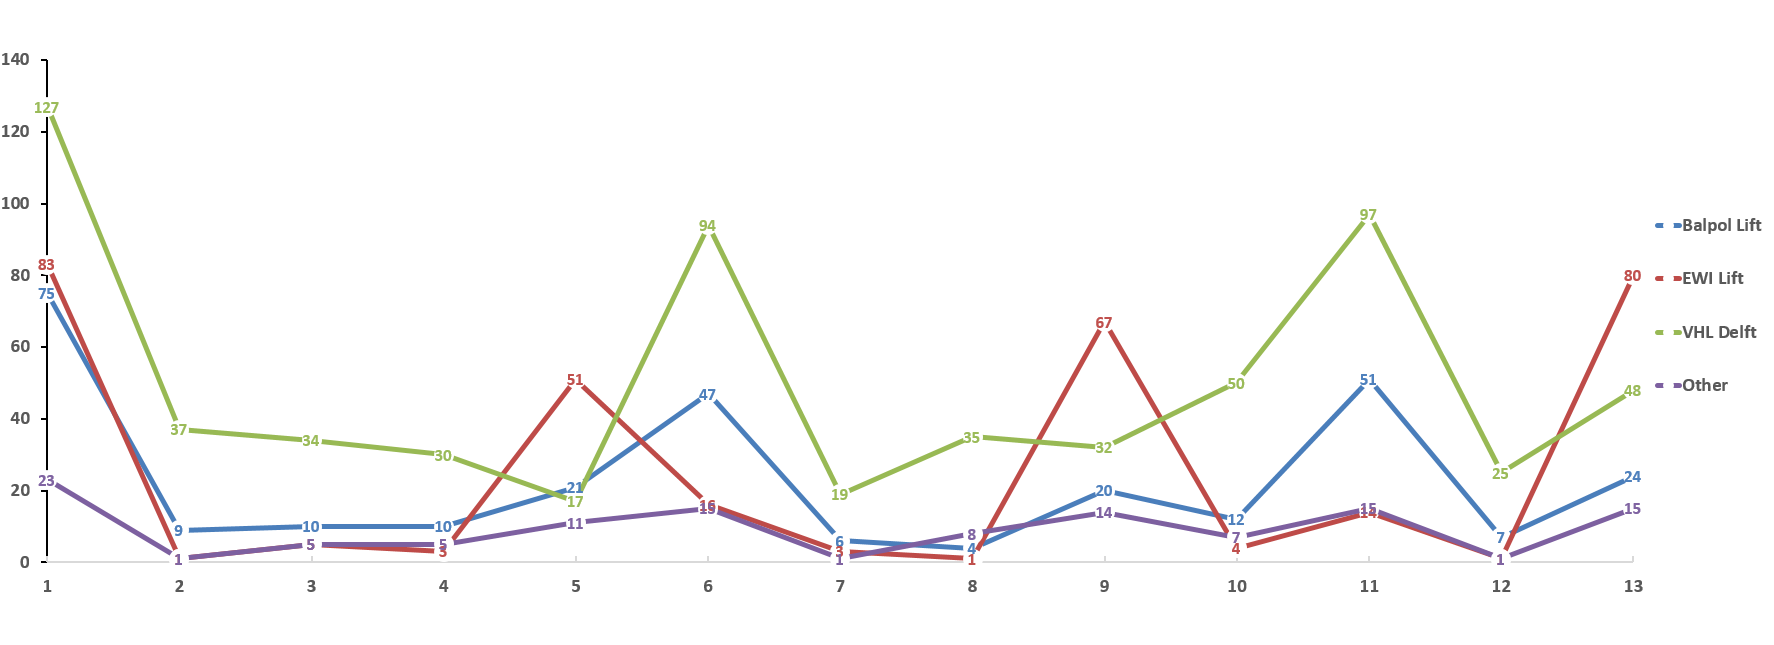
\includegraphics[scale=0.3]{static_per_channel_graph3.png}
\caption{SSIDs per channel for different static situations. $T_{dwell}=250ms$}
\label{fig:static_per_channel_graph}
\end{figure}
In Figure \ref{fig:static_per_channel_graph} we compare different static situations, a clear difference can be seen between the campus (EWI Lift) and residential buildings (VHL Delft and Balpol Lift).
Where on the campus there is a clearly managed network of AP's on specific channels (1, 5, 9 and 13). While this is also somewhat the case for the residential buildings where channels 1, 6 and 11 are often used, we also see non standard channels more often being used. This difference can be explained by the fact that in residential area's people configure AP's themselves and often pick a channel that seems logical on the day of the installation, not taking into account that it's recommend to go for 1 of the orthogonal channels\footnote{Channels which barely overlap in the frequency space}. While in the professionally configured network of the campus it is clear that this knowledge is present when installation is done and the better channels are chosen.

\subsection{Dynamic measurements}
\begin{figure}[h!]
\centering
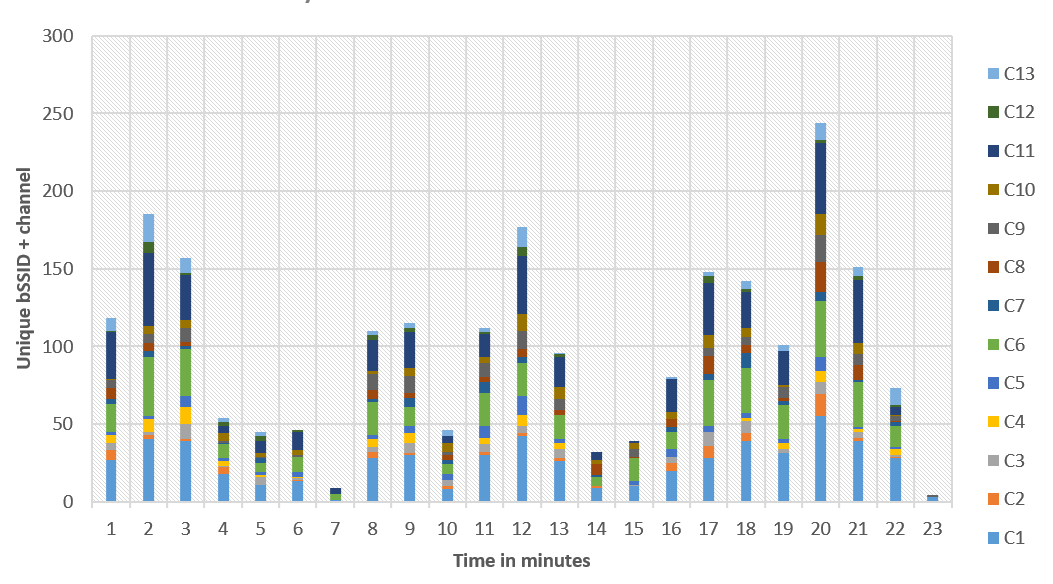
\includegraphics[scale=0.45]{NoncumuDynamicGraph.png}
\caption{Unique amount of BSSID's per channel per time bin of 60 seconds. ($T_{dwell}=100ms$)}
\label{fig:dynamic_zoetermeer_aula}
\end{figure}
For the dynamic measurements we chose to capture on public bus transportation since we already needed to travel and it is possible to use your laptop while traveling also the limited speed of the bus is favourable as opposed to car or train. In Figure \ref{fig:dynamic_zoetermeer_aula} you can see the channel distribution of a bus ride. Clear differences can be seen between rural areas(4-7 minute\footnote{Between Zoetermeer and Pijnacker}) and more densely populated areas (11-13 minute\footnote{Centre of Pijnacker} and 17-22 minute\footnote{In Delft}) in the amount of AP's visible. While we only show 1 graph here and the cumulative version, the same behaviour is seen over different measurements on different routes. As we already noted in the static measurements, channels 1, 6 and 11 are the most used channels in residential areas. We see this again in this dynamic measurement (Figure \ref{fig:dynamic_zoetermeer_aula_cumu} shows this accumulation).

\begin{figure}[h!]
\centering
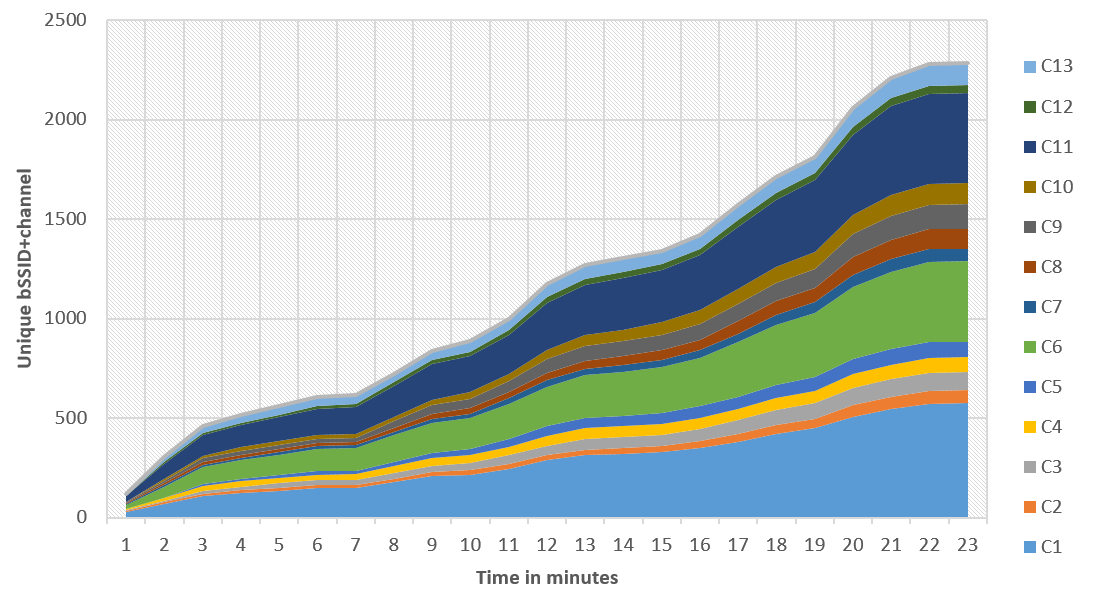
\includegraphics[scale=0.45]{ChosenGraphDynamic.png}
\caption{Cumulative amount of BSSIDs per channel for a bus drive from Zoetermeer to TU Aula, data aggregated in time bins of 1 minute. ($T_{dwell}=100ms$)}
\label{fig:dynamic_zoetermeer_aula_cumu}
\end{figure}

\section{Conclusion}
From the data we clearly see that there is a preference for certain wifi channels, namely 1, 6 and 11. However we can see that certain large managed installations can greatly deviate from these defaults. Furthermore we can see that there is strong correlation between the amount wifi AP's and how densely populated an area is.


\end{document}
